\documentclass[11pt, oneside]{article}   	% use "amsart" instead of "article" for AMSLaTeX format
\usepackage{geometry}                		% See geometry.pdf to learn the layout options. There are lots.
\geometry{letterpaper}                   		% ... or a4paper or a5paper or ... 
%\geometry{landscape}                		% Activate for for rotated page geometry
%\usepackage[parfill]{parskip}    		% Activate to begin paragraphs with an empty line rather than an indent
\usepackage{graphicx}				% Use pdf, png, jpg, or eps� with pdflatex; use eps in DVI mode
								% TeX will automatically convert eps --> pdf in pdflatex		
\usepackage{amssymb}
\usepackage{amsmath}
\usepackage{parskip}

\title{Critical points}
%\author{The Author}
%\section{}
% \subsection*{R code}
\date{}							% Activate to display a given date or no date

\graphicspath{{/Users/telliott_admin/Dropbox/Tex/png/}}

\begin{document}
\maketitle
\Large
%\noindent

A major application of derivatives is in the computation of values of the independent variable ($x$) where a function $y = f(x)$ takes on either a maximum or minimum value.  Such points are called critical points, and these points may be either a \emph{local} or \emph{absolute} max/min.

By definition, a critical point is a value in the function's domain where its derivative (slope) is zero.  For example, the parabola
\[ (y-1) = (x-1)^2 \]
(shifted from the origin to make things a little more interesting), can be rearranged to yield
\[ y = x^2 - 2x + 2 \]
\[ y' = 2x - 2 \]

Set it equal to zero:
\[ 0 = 2x - 2 \]
\[ x = 1 \]

The derivative $y'$ is zero when $x=1$, and at that point $y=1$.  As you should recognize from the first equation, this is the vertex of the parabola.  Furthermore, the second derivative
\[ y'' = 2 \]
is positive.  What this means is that the rate of change of the slope is everywhere positive for this function, it starts out negative, becomes zero at the critical point, and then becomes positive.

Every maximum or minimum is a critical point, where the slope of $f(x)$ is zero.  However, the converse is not true.  Some critical points are not extrema.  For example

\[ y = x^3 \]

\begin{center} 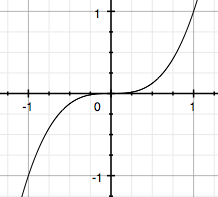
\includegraphics [scale=0.5] {y=x^3.png} \end{center}

The slope of this function is $y' = 3x^2$ and it is zero only at $x=0$.  But the slope can never be negative, because of the $x^2$ part.  

\subsection*{cubic equation}

Now consider the function
\[ y = x^3 - 4x \]

Take the derivative
\[ y' = 3x^2 - 5 \]
Set it equal to zero:
\[ 0 = 3x^2 - 5 \]
\[ x = \sqrt{\frac{5}{3}} \approx \pm \ 1.29 \]
\[ y \approx \pm \ 3.012 \]

We have two critical points, symmetric about the $y$-axis.

These aren't particularly "nice" values but that's OK.  The equation was set up to make it easy to find the roots (zeroes), which can be done by factoring

\[ y = x(x+2)(x-2) \]

The graph of this function 

\begin{center} 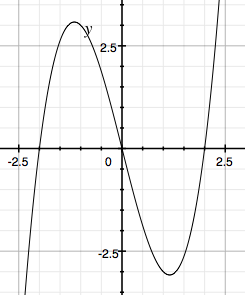
\includegraphics [scale=0.5] {y=x^3-4.png} \end{center}

crosses the $x$-axis at $x=-2,0,2$.  At the first point, the slope is positive, at the second negative.  The critical point at $x=-\sqrt{5/3}$ is a maximum.  We can also see this analytically since

\[ y'' = 6x \]

Since $y'' < 0$ at the first critical point, it is a maximum.  By similar logic, the second point is a minimum.

In some cases it is possible that the second derivative is difficult to compute or evaluate.  One can simply look at the slope a little for $x$ slightly smaller or larger than the critical value, and see how it's changing, to determine whether the point is a minimum or a maximum.

\subsection*{Issues}

In addition to the critical points, it is also necessary to evaluate the endpoints of the function's domain $[\ a,b\ ]$.

Also, it is possible that the max or min values occur as the function goes to $\infty$.  In that case, we do not say that the function has a min/max at infinity, since this is not a number.

Another point is that if the function has issues, one needs to look at those points.  For example, the absolute value function is continuous but is not differentiable at $x=0$, and this is a minimum for the function.

Finally, if a function is not continuous all bets are off.  For example 
\[ y = \frac{x}{x-1} \]

\begin{center} 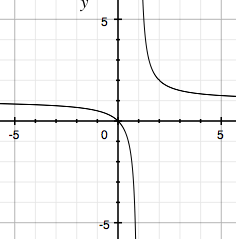
\includegraphics [scale=0.5] {x_x-1.png} \end{center}

has its max and min as $x \rightarrow 1+$ and $x \rightarrow 1-$.  And of course, any function defined like this has issues:

 \begin{displaymath}
   f(x) = \left\{
     \begin{array}{lr}
       1-x & : x < 0 \\
       1 & : 0 \le x \le 1 \\
       x & : x > 1
     \end{array}
   \right.
\end{displaymath} 

Here, the minimum is the entire domain between $0$ and $1$, an infinite number of points.




\end{document}  